\usepackage[german]{babel}
\usepackage[utf8]{inputenc}
\usepackage{times}
\usepackage[T1]{fontenc}
\usepackage{eurosym}
\usepackage{graphicx}
\usepackage{amsmath}
\usepackage[siunitx,european]{circuitikz}
\usepackage{ulem}
\usepackage{listings}
%
\lstset{numbers=left, numberstyle=\tiny, stepnumber=2, numbersep=5pt, language = C++, alsolanguage=XML}
% \MyLogo{\includegraphics[height=1cm]{../../../../bilder/bwslogo_3.png}}
% % \includegraphics{../../bilder/bwslogo_3.png}
% % bwslogo_3.png: 476x392 px, 300dpi, 4.03x3.32 cm, bb=
%
\only<article>{
\usepackage[colorlinks=true,linkcolor=blue,filecolor=magenta,urlcolor=cyan]{hyperref}
}

\only<presentation>{
  \usepackage{hyperref}
}


\title{Arbeitsunterlagen zu FOS Elektrotechnik Themenfeld 12.6}
\subtitle{Elektrisches und magnetisches Feld}
\date{V 0.1.0 - im Aufbau\\ Stand: \today}%\\

\institute[BWS Hofheim]{Brühlwiesenschule, Hofheim}
\author{Thomas Maul}

\titlegraphic{Für eigene Teile gilt: 
\includegraphics[height=1cm]{cc_by-nc_eu.png}}

\begin{document}
\only<article>{
\maketitle
\tableofcontents
\clearpage
}
\begin{frame}<beamer>
  \titlepage
  % \hyperlink{Teil_2}{\beamerbutton{Go part 2}}
\end{frame}
% \AtBeginSection[] % Do nothing for \section*
% {
%   \begin{frame}<beamer>
%     \frametitle{Inhalt}
%     \tableofcontents[currentsection]
%   \end{frame}
% }


% \part{Themenfeld 12.6 - Elektrisches und magnetisches Feld}
% \label{Teil_12_6}
\begin{frame}
  \partpage
  %   \tableofcontents[hidesubsections]
\end{frame}

\begin{frame}
  \partpage
\end{frame}
\begin{frame}<beamer>
  \frametitle{Inhalt}

  \begin{columns}
    \column{.5\textwidth}
    \tableofcontents[sections={7-12}]%currentsection]
    \column{.5\textwidth}
    \tableofcontents[sections={13-}]%currentsection]
  \end{columns}

\end{frame}

\section{Ladungen, Kräfte}
\only<presentation>{
  \begin{frame}{Elektronen und Atome}
    \begin{itemize}
      \item Die Materie besteht aus Atomen.
      \item Kern: Protonen und Neutronen, Hülle: Elektronen
      \item Bei Leitern: Elektronen \glq mobil\grq, bei Nichtleitern fest(er)
      \item Reibung von 2 Nichtleitern (Stoff und Glasstab)$\Rightarrow$ Ladungstrennung
    \end{itemize}
  \end{frame}
}
Die Materie besteht aus Atomen. Diese wiederum aus einem Kern mit Protonen und Neutronen und einer Hülle aus Elektronen. Bei einigen Atomen, zum Beispiel Metalle sind, ist es leicht möglich einzelne Elektronen aus der Hülle zu entfernen. Dies führt zur elektrischen Leitung - dem elektrischen Strom. Bei Stoffen, die nicht leitend sind, lassen sich die Elektronen nicht oder nur schwer aus der Hülle entfernen.

Wenn man zwei nicht leitende Gegenstände, zum Beispiel einen Glasstab und ein Stück Stoff aneinander reibt, werden durch die Reibung Elektronen in einem der beiden Gegenstände aus der Hülle herausgerissen und in die Atomhüllen der Atome des anderen Gegenstands übertragen. In diesem Moment spricht man davon, dass beide Gegenstände elektrisch geladen sind.
\begin{frame}{Katze mit Styroporflocken}
  \begin{figure}[htb]
    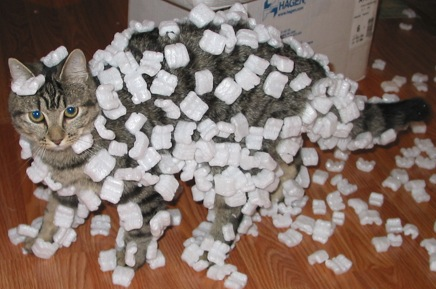
\includegraphics{Cat_demonstrating_static_cling_with_styrofoam_peanuts.jpeg}
    %    Cat_demonstrating_static_cling_with_styrofoam_peanuts.jpeg: 436x289 px, 180dpi, 6.15x4.08 cm, bb=
    \caption{Katze mit Styroporflocken}
    \label{abb:CatWidthStyropor}
    \end{figure}
  \footnote{Quelle: Von Original image: Sean McGrath from Saint John, NB, CanadaDerived image: Black Rainbow 999 - Diese Datei ist ein Ausschnitt aus einer anderen Datei, CC BY 2.0, https://commons.wikimedia.org/w/index.php?curid=60287175}
\end{frame}

\only<presentation>{
  \begin{frame}{Anziehung und Abstoßung von Ladungen}
    \begin{itemize}
      \item gleichnamige Ladungen stoßen sich ab.
      \item ungleichnamige Ladungen ziehen sich an.
      \item bei Elektrostatik gibt es keine Bewegung, nur Kräfte
    \end{itemize}
  \end{frame}
}

Elektrische Ladungen, die gleich sind (zwei positive Ladungen oder zwei negative) stoßen sich ab. Ladungen, die unterschiedlich sind, ziehen sich an. Die Abstoßung und Anziehung kann man als Kräfte berechnen und in gewissen Grenzen messen.

Wenn sich die Ladungen nicht zwischen den Körpern bewegen und auch nicht innerhalb des Körpers, nennt man dies einen statischen Zustand. Die Ladung ist vorhanden, die Kräfte sind vorhanden aber es gibt keine Bewegung. Unter idealen Bedingungen bleibt der Zustand dauerhaft bestehen. In der Schule vereinfachen wir. Eine Ladung ist als punktförmig definiert, sie hat keine Ausdehnung, für die Elektrostatik gilt, dass sie ohne äußere Einflüsse unverändert bleibt. Elektronen und Ladungen bewegen sich nicht.

\section[Energieerhaltung]{Energieerhaltung und Einheit}
\only<presentation>{
\begin{frame}
  \frametitle{Inhalt}

%  \begin{columns}
%    \column{.5\textwidth}
    \tableofcontents%[sections={7-12},currentsection]
%    \column{.5\textwidth}
%    \tableofcontents[sections={13-},currentsection]
%  \end{columns}
\end{frame}
}

\only<presentation>{
  \begin{frame}{Energieerhaltung und Einheit}
    \begin{itemize}
      \item Energieerhaltung
      \item Elektrische Ladung Coulomb (C) gemessen
      \item $1 C = 1 As$. \
      \item Elementarladung $e = 1,602 * 10^{-19} C$
      \item Kräfte zwischen Ladungen
      \item Anziehung (+ > < -) und \\Abstoßung (+ < > +), (- < > -)
    \end{itemize}
  \end{frame}
}
Unabhängig von den Vereinfachungen gilt, dass es einen Energieerhaltungssatz gibt. Energie kann nur umgewandelt werden. Potentielle in kinetische oder chemische Energie. Energie kann innerhalb eines geschlossenen Systems (wir gehen davon aus, dass unsere System alle geschlossen sind) nicht entstehen und nicht vernichtet werden. Damit bleibt die Gesamtladung auch immer identisch. Die Elektrische Ladung wird in Coulomb (Einheit C) gemessen, $1 C = 1 As$. \\ Die Elementarladung (kleinste Einheit) beträgt: $e = 1,602 * 10^{-19} C$

Wenn eine positive Ladung und eine negative Ladung nahe beieinander existieren, bilden sich zwischen ihnen Kräfte. Zusätzlich kann man ein elektrostatisches Feld messen. Das Feld wird als Linien dargestellt. Die Feldlinien beginnen bei der positiven Ladung und enden an der negativen Ladung.

\section[Ladungen]{Abmaße von Ladungen}
\only<presentation>{
\begin{frame}
  \frametitle{Inhalt}

% \begin{columns}
%    \column{.5\textwidth}
    \tableofcontents%[sections={7-12},currentsection]
%    \column{.5\textwidth}
%    \tableofcontents[sections={13-},currentsection]
%  \end{columns}
\end{frame}
}

% \only<presentation>{
\begin{frame}{Abmaße von Ladungen}
  \begin{description}
    \item[Punktlandung] unendlich klein
    \item[Linienladung] dünne Linie, z.B. Draht
    \item[Flächenladung] gleichmäßig auf der Fläche
    \item[Raumladung] gleichmäßig im Raum
  \end{description}
\end{frame}
% }
Eine Punktladung wird als unendlich kleiner Punkt definiert. Wichtig ist, dass der Durchmesser der Ladung wesentlich kleiner ist, als der Abstand zu einer anderen Ladung.

Eine Linienladung stellt eine Linie dar, auf der sich die (gleichnamigen) Ladungen befinden. Die Linie ist relativ gesehen dünn, es kann zum Beispiel ein Draht sein, der im Raum als Linie dargestellt werden kann. Die Ladungen sind gleichmäßig auf der kompletten Strecke verteilt.

Eine Flächenladung verteilt sich auf einer Fläche gleichmäßig. In der Regel passiert dies bei metallischen Flächen oder anderen Flächen, die gut leitend sind. Hier verteilen sich die Ladungen auf der gesamten Fläche gleichmäßig.

Eine Raumladung stellt eine gleichmäßige Verteilung elektrischer Ladungen innerhalb eines Volumens dar.

\section{Vektoren}
\only<presentation>{
\begin{frame}<beamer>
  \frametitle{Inhalt}

%  \begin{columns}
%    \column{.5\textwidth}
    \tableofcontents%[sections={7-12},currentsection]
%    \column{.5\textwidth}
%    \tableofcontents[sections={13-},currentsection]
%  \end{columns}
\end{frame}
}

Ein Vektor beschreibt den Abstand und die Richtung zwischen zwei Punkten. In Bild \ref{fig:ZweiVektoren} sind zwei Vektoren: $\vec{v}_1= \left(\begin{array}{c} 1 \\ 2 \end{array}\right)$ und  $\vec{v}_2= \left(\begin{array}{c} 2 \\ 1 \end{array}\right)$. Jeder Vektor beschreibt einen Punkt im Koordinatensystem. Der Startpunkt des Vektors muss nicht im Punkt $\left(\begin{array}{c}0\\0\end{array}\right)$ sein. Daher beschreibt der Vektor eine Verschiebung eines Punkts um die Koordinaten (hier x und y).

Die Länge des Vektors, der sogenannte Betrag, wird mit der $\sqrt{\Delta x^2 + \Delta y^2}$ berechnet. Hier: \[|v_1| = \sqrt{(1 - 0) + (2 - 0)} = \sqrt{3}\].
\begin{frame}{Vektoren}
  \begin{figure}[htb]
    \begin{tikzpicture}
      \draw (-2,0) -- (2,0);
      \draw (0,-2) -- (0,2);
      %\draw node[circ] at (0,0){};
      \draw[->] (0,0) -- (1,2);
      \draw[->] (0,0) -- (2,1);
      \draw node at (0.8,1) {$\vec{v}_1$};
      \draw node at (1.4,0.4) {$\vec{v}_2$};
    \end{tikzpicture}

    $\vec{v}_1= \left(\begin{array}{c} 1 \\ 2 \end{array}\right)$ und  $\vec{v}_2= \left(\begin{array}{c} 2 \\ 1 \end{array}\right)$
    \caption{Zwei Vektoren in zweidimensionalen Raum}
    \label{fig:ZweiVektoren}
  \end{figure}
\end{frame}

Vektoren können addiert werden, dabei werden jeweils die X-Komponenten, Y-Komponenten und ggf. weitere Komponenten einzeln addiert.
\begin{align}
  \vec{v}_3 &= \vec{v}_1 + \vec{v}_2\\
  \vec{v}_3 &= \left(\begin{array}{c} 1 \\ 2 \end{array}\right) + \left(\begin{array}{c} 2 \\ 1 \end{array}\right)\\
  \vec{v}_3 &= \left(\begin{array}{c} 3 \\ 3 \end{array}\right)
\end{align}

\begin{frame}{Addition von Vektoren}
  \begin{figure}[htb]
    \begin{tikzpicture}
      \draw (-2,0) -- (2,0);
      \draw (0,-2) -- (0,2);
      %\draw node[circ] at (0,0){};
      \draw[->] (0,0) -- (1,2);
      \draw[->] (0,0) -- (2,1);
      \draw[->] (1,2) -- (3,3);
      \draw[->] (0,0) -- (3,3);
      \draw node at (0.9,1.2) {$\vec{v}_1$};
      \draw node at (1.4,0.4) {$\vec{v}_2$};
      \draw node at (1.6,2) {$\vec{v'}_2$};
      \draw node at (2,1.5) {$\vec{v}_3$};
    \end{tikzpicture}

    $\vec{v}_1= \left(\begin{array}{c} 1 \\ 2 \end{array}\right)$, $\vec{v}_2= \left(\begin{array}{c} 2 \\ 1 \end{array}\right)$, $\vec{v'}_2 = \vec{v}_2$  und $\vec{v}_3= \left(\begin{array}{c} 3 \\ 3 \end{array}\right)$
    \caption{Zwei Vektoren in zweidimensionalen Raum}
    \label{fig:ZweiVektorenAddiert}
  \end{figure}
\end{frame}

\only<presentation>{
  \begin{frame}{Kraft als Vektor, Spannung}
    \begin{itemize}
      \item Kraft $\widehat{=}$ Vektor
      \item Richtung, Betrag
      \item Addition
      \item Spannung $\widehat{=}$ Spannung zwischen 2 Punkten
      \item auch im Raum (E-Feld)
    \end{itemize}
  \end{frame}
}
\section[E-Feld]{Elektrische Feldstärke}
\only<presentation>{
\begin{frame}
  \frametitle{Inhalt}

%  \begin{columns}
%    \column{.5\textwidth}
    \tableofcontents%[sections={7-12},currentsection]
%    \column{.5\textwidth}
%    \tableofcontents[sections={13-},currentsection]
%  \end{columns}
\end{frame}
}



\section[Überlagerung E]{Überlagerung von elektrischen Feldern}
\only<presentation>{
\begin{frame}
  \frametitle{Inhalt}

  \begin{columns}
    \column{.5\textwidth}
    \tableofcontents[sections={7-12},currentsection]
    \column{.5\textwidth}
    \tableofcontents[sections={13-},currentsection]
  \end{columns}
\end{frame}
}

\section{Pflicht-Themen, die noch offen sind}
\begin{frame}{Pflicht-Themen, die noch offen sind}
Folgende Themen sind gemäß Prüfungserlass für die Prüfung 2026 Pflicht, aber noch nicht ausgearbeitet.
\begin{itemize}
    \item Kondensator
    \\ Auf- und Entladung
    \item Induktion
    \\ Magnetischer Fluss (Phi)
    \\ Flussdichte (B) 
    \item Spule
    \\ Ein- und Ausschaltvorgang 
\end{itemize}

Die Themen folgen demnächst hier.
\end{frame}

% \section[Kondensator]{Kondensator (Pflicht)}
% \only<presentation>{
% \begin{frame}
%   \frametitle{Inhalt}
% 
%   \begin{columns}
%     \column{.5\textwidth}
%     \tableofcontents[sections={7-12},currentsection]
%     \column{.5\textwidth}
%     \tableofcontents[sections={13-},currentsection]
%   \end{columns}
% \end{frame}
% }
% \subsection[C laden]{Auf- und Entladung (Pflicht)}
% 
% \section[Induktion]{Induktion (Pflicht)}
% \only<presentation>{
% \begin{frame}
%   \frametitle{Inhalt}
% 
%   \begin{columns}
%     \column{.5\textwidth}
%     \tableofcontents[sections={7-12},currentsection]
%     \column{.5\textwidth}
%     \tableofcontents[sections={13-},currentsection]
%   \end{columns}
% \end{frame}
% }
% 
% \subsection[Phi]{Magnetischer Fluss (Phi) (Pflicht)}
% \subsection[B]{Flussdichte (Pflicht)}
% 
% \section[Spule]{Spule (Pflicht)}
% \only<presentation>{
% \begin{frame}
%   \frametitle{Inhalt}
% 
%   \begin{columns}
%     \column{.5\textwidth}
%     \tableofcontents[sections={7-12},currentsection]
%     \column{.5\textwidth}
%     \tableofcontents[sections={13-},currentsection]
%   \end{columns}
% \end{frame}
% }
% 
% \subsection{Ein- und Ausschaltvorgang (Pflicht)}
